\documentclass[preprint]{vgtc}

\usepackage{times}
\renewcommand*\ttdefault{txtt}
\usepackage{mathptmx}

\usepackage{xcolor}
\usepackage{multicol}
\usepackage{notation}
\usepackage{wrapfig}
\usepackage{multirow}
\usepackage{hyperref}
\usepackage{caption}

\usepackage{graphicx}
\usepackage{amsmath,amssymb}

\usepackage{lipsum}
\graphicspath{{../paper/figures/}{figs}}

\onlineid{0}
\vgtccategory{Research}
%\vgtcinsertpkg




\title{Topological Equivariant Artist Model}

\author{
Hanna Aizenman\thanks{e-mail: haizenman@gradcenter.cuny.edu} \\
\scriptsize{CUNY Graduate Center}
\and
Mikael Vejdemo-Johansson\thanks{e-mail: mvj@math.csi.cuny.edu} \\
\parbox{1.6in}{\scriptsize \centering CUNY College of Staten Island \\
CUNY Graduate Center}
\and
Thomas Caswell\thanks{e-mail: tcaswell@bnl.gov} \\
\parbox{1.8in}{\scriptsize\centering National Synchrotron Light Source II \\ Brookhaven National Lab}
\and
Michael Grossberg\thanks{e-mail: mgrossberg@ccny.cuny.edu} \\
\parbox{1.6in}{\scriptsize\centering City College of New York \\ CUNY Graduate Center}
}

%\keywords{TODO:list keywords}

\abstract{
    The contract data visualization tools make with their users is that a chart is a faithful and accurate visual representation of the numbers it is made from. Motivated by wanting to make better tools, we propose a methodology for fully specifying arbitrary data to visualization mappings in a manner that easily translates to code. We propose that fiber bundles provide a uniform interface for describing a variety of underlying data - tables, images, networks, etc. - in a manner that independently encodes the mathematical structure of the topology and the fields of the dataset. Modeling the data structures that store the datasets as sheaves provide a method for specifying visualization methods that are designed to work regardless of how the dataset is stored - whether the data is on disk, distributed, or on demand. Specifying the visualization library components as natural transforms of sheaves means that the constraints that the component must satisfy to be structure preserving can be specified as the set of morphisms on the data and graphic sheaves, including the structure on the topology and fields of the data.
    Using category theory to formally express how visual elements are constructed means we can translate those expectations into code, which can then be used to enforce the expectation that a visualization tool is faithfully translating between numbers and charts.
    The sheaf formalism is generic enough that with appropriate choices of a sheaf structure to replace the graphic sheaves, the same framework will work to model and specify non-visual modalities with identical underlying data representations, and structurally similar data to perception transformations.
}

\begin{document}

\maketitle

\section{Intro}
\label{sec:intro}

\begin{figure}
\begin{center}
    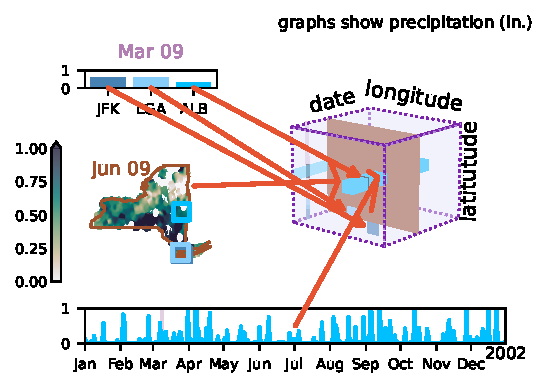
\includegraphics[width=3.5in]{k_different_types.pdf}
\end{center}
\caption{This weather station data has multiple embedded continuities - points at each time and position, timeseries at each position, and maps at each time - that are expected to be homeomorphic to the continuity of their respective visualizations.}
    \label{fig:homeomorphism}
\end{figure}
Motivated by wanting to make better tools, we propose a methodology for fully specifying arbitrary data to visualization mappings in a manner that easily translates to code. Generally, preserving structure means that a visualization is expected to preserve the $field$ properties and $topology$ of the corresponding dataset, where \textcolor{fiber}{\textbf{field}} is a set of values of the same type and \textcolor{base}{\textbf{topology}} is the connectivity and relative positioning of elements in a dataset \cite{wilkinsonGrammarGraphics2005}.  Field structure is traditionally codified as the Steven's measurement scales \cite{stevensTheoryScalesMeasurement1946}, where each scale is a set of actions on a group. Topological structure is generally assumed by visual algorithms \cite{chiTaxonomyVisualizationTechniques2000, toryRethinkingVisualizationHighlevel2004}, but generally do not verify that input structure.
For example, a \texttt{line} algorithm often does not have a way to query whether a list of (x,y) coordinates is the distinct rows, the time series, or the list of stations in \autoref{fig:homeomorphism}. We propose that the bar plot, line plot, and heatmap can be verified as structure preserving because they have a homeomorphic relationship to the 0D ($\bullet$) points, 1D (--) linear, and 2D ($\blacksquare$) surface continuities embedded in the continuous 3 dimensional. Our methodology generalizes Bertin\cite{bertinSemiologyGraphicsDiagrams2011}'s codification of structure,  Mackinlay\cite{mackinlayAutomaticDesignGraphical1987} mathematical formalization, Wilkinson's set theoretic approach \cite{wilkinsonGrammarGraphics2005}, and Kindlemann and Scheidegger's algebraic visualization design (AVD) framework \cite{kindlmannAlgebraicProcessVisualization2014} by explicitly incorporating topology, supporting non-group and non-monoidal structures, and by providing a framework for translating the theoretical ideas into buildable components.

Through this paper we will be discussing visualization primarily, but by changing the last of the three fiber bundles we discuss in Section~\ref{sec:data models}, we could go from a visual representation to an auditory, haptic, or any other modality and retain the benefits we identify from the fiber bundle and sheaf structures.


\section{Data Model}
\label{sec:data models}

Spivak represents relational databases with a fiber bundle representation \cite{spivakDatabasesAreCategories2010,spivakSimplicialDatabases2009}. This suggests a way for us to extend Butler's proposal of using fiber bundles as an abstraction for visualization data \cite{butlerVectorBundleClassesForm1992,butlerVisualizationModelBased1989} by incorporating Spivak's approach, and extending it from data storage to represent the transformation to graphical representation. As we show in Table~\ref{tab:data_abstraction}, where Spivak represents a specific dataset as a fiber, a database schema with the bundle's fiber space and topological indexing through a base space, we introduce parallel analogous structures representing a visual specification and a graphic realization.

\begin{figure}
%\begin{multicols}{2}
    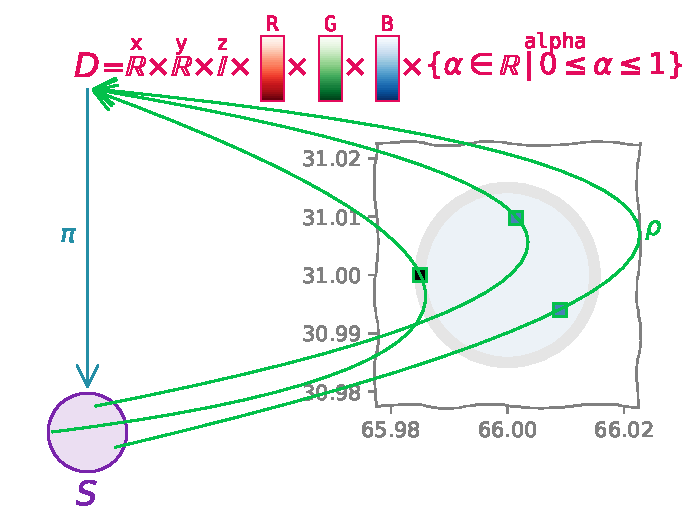
\includegraphics[width=.5\textwidth]{fb_rho.pdf}
%    \columnbreak
    \caption{The scatter marker is specified by the section $\gsection$, which maps into the fiber $\gfiber$ to retrieve the values that compose into the pixel (approximated as a square) returned by the section function evaluated at each point $\gbasepoint$. The section evaluated over the entire space $\gsection\vert_{S}$ returns the entire scatter mark, shown here in faded form to make it easier to see the individual pixels.}\label{fig:fiber_bundle}
\end{figure}


\begin{table*}[t]
    \begin{tabular}{|r | c c c|}
    \hline
     structure/abstraction & Data & Visual & Graphic\\
    \hline
\textcolor{fiber}{fiber}/\textcolor{total}{total}\ /\textcolor{base}{base} spaces &   \multirow{2}{*}{$\dfiberc \hookrightarrow \dtotalc \xrightarrow{\pi} \dbasec$} &   \multirow{2}{*}{$\vfiberc \hookrightarrow \vtotalc \xrightarrow{\pi} \dbasec$} &  \multirow{2}{*}{$\gfiberc \hookrightarrow \gtotalc \xrightarrow{\pi} \gbasec$}\\
fields/datasets/topology&&&\\
\hline
\textcolor{base}{point}/\textcolor{base}{openset}/\textcolor{base}{base space} &  \multirow{2}{*}{$\dbasepointc \in \opensetc \subseteq \dbasec$} & \multirow{2}{*}{$\dbasepointc \in \opensetc \subseteq \dbasec$} & \multirow{2}{*}{$\gbasepointc \in \opensetgc \subseteq \gbasec$}\\
index/subset/indices & & & \\
\hline
\textcolor{fiber}{fiber space}  record/fields &  $\delementc \in \dfiberc$ & $\velementc \in \vfiberc$ & $\gelementc \in \gfiberc$ \\
\hline
\textcolor{section}{section} dataset & $\cgamma{\dbasec}{\dtotalc} \ni \dsectionc: \dbase \textcolor{section}{\rightarrow} \dfiberc$ & $\cgamma{\dbasec}{\vtotalc} \ni \vsectionc: \dbase \textcolor{section}{\rightarrow} \vfiberc$ &  $\cgamma{\gbasec}{\gtotalc} \ni \gsectionc: \gbase \textcolor{section}{\rightarrow} \gfiberc$ \\
\hline
\textcolor{sheaf}{sheaf} data container  &  \multirow{2}{*}{$\sheafc_{\dbasec, \dtotalc}: \opensetc \rightarrow \cgamma{\opensetc}{\dtotalc\restriction_{\opensetc}}$} &  \multirow{2}{*}{$\sheafc_{\dbasec, \vtotalc}: \opensetc \rightarrow \cgamma{\opensetc}{\vtotalc\restriction_{\opensetc}}$} &   \multirow{2}{*}{$\sheafc_{\gbasec, \gtotalc}: \opensetgc \rightarrow \cgamma{\opensetc}{\gtotalc\restriction_{\opensetgc}}$} \\
&&&\\
        \hline
    \end{tabular}
    \caption{Summary of how the data is abstracted using topological structures}
    \label{tab:data_abstraction}
\end{table*}

By choosing a topological space $\mathcal T$ as indexing space underlying the dataset we get a uniform abstraction for describing arbitrary continuity -- time series, lists of observations, spatial fields all have the same abstract structure -- and we get a method for managing overlapping embedded topologies, such as we show in \autoref{fig:homeomorphism}. Spivak's fiber bundle construction of types decouples field types from field names and single-dimensional and multi-dimensional fields share a common abstraction: they all rely on some choice of mathematical object for the data types. A particular dataset can in this paradigm be encoded as a \textcolor{section} \dsectionc\ of a bundle, assigning to each index value an observation in the data types prescribed by the fiber space. This fits topology and field types into a data definition $\textcolor{section}{\texttt{dataset}}: \textcolor{base}{\texttt{topology}} \rightarrow \textcolor{fiber}{\texttt{field}}$.

We abstract these data containers as sheaves, and the gluing property of sheaves provides a systematic way to track continuity of the data \cite{ghristElementaryAppliedTopology2014} and apply visual algorithms developed on this model regardless whether the data fits in memory, is distributed, or streaming.

\section{Artist}
\label{sec:Artist}

We call the mapping from data to graphic $\vartistc:\dsectionc\mapsto\gsectionc$ an \textcolor{artist}{Artist}\footnote{Artists are named for the Artist class in Matplotlib. Artist is the parent class of all the objects that assemble and manage visual elements such as points, lines, and shapes.}. 
Artists are structure preserving when they are implemented as sheaf maps from the data representation sheaf to the graphics sheaf. This means that the artist satisfies the following constraints, as illustrated in \autoref{fig:artist}:

\begin{figure}
    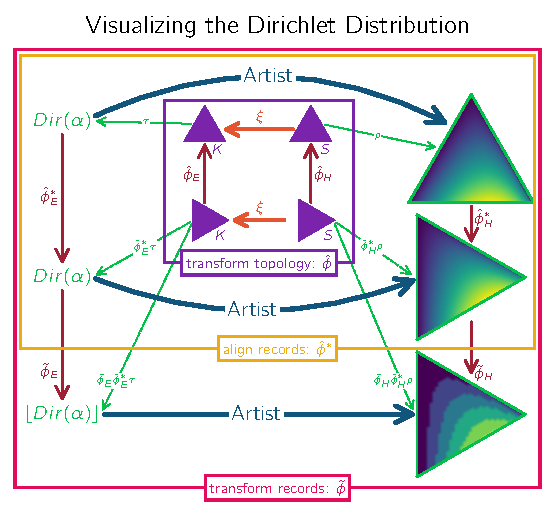
\includegraphics[width=.5\textwidth]{artist_equiv.pdf}
    \caption{}\label{fig:artist}
\end{figure}

\begin{description}
    \item[homotopic] there exists a deformation retract\footnote{This requirement emerges from the digital geometry nature of displays: even if the intended visual primitive may be 1-dimensional, it's screen realization must be 2-dimensional -- requiring a deformation retract most closely agrees with our intuition for drawing geometric primitives} $\vindexc: \gbasec\rightarrow\dbasec$ between graphic and artist base space
    \item[topology] the artist is commutative w.r.t. the presheaf morphism $\dfunchc: \dbasepointc^{\prime}\mapsto \dbasepointc$ and pullback $\dfuncpullc \dsectionc \restriction_{\opensetc^{\prime}}: \dsectionc\restriction_{\opensetc^{\prime}} \mapsto \dsectionc \restriction_{\opensetc^{\prime} \circ \dfunchc}$: index changes on the record leaves values in the record unmodified
    $\dsectionc(\dbasec) = \dfuncpullc\dsectionc(\dbasepointc^{\prime}) = \dsectionc(\dfunchc(\dbasepointc^{\prime}))$
    \item[fields] the artist is commutative w.r.t. actions on the fiber. An action $\dfunctc: \dfiberc\to\dfiberc$ induces a function between sections $\dfunctc: \dfuncpullc \dsectionc \restriction_{\opensetc^{\prime}} \mapsto \dfuncpullc \dsectionc^{\prime} \restriction_{\opensetc}$. We also require $\dfunctc$ to respect the structure, such as operators, of $\dfiber$.
\end{description}

With this underlying topological structure to describe the visualization pipeline, traditional constructions from topology and category theory generate natural operators on the data structures. Pushouts and pullbacks, of central importance in category theory and topology, emerge here as operators to add and extend records, respectively. Since (in categorical language) sheaf maps preserve limits and colimits, this observation shows that artists are composable: $\vartistc(\bigsqcup\limits_{i}\dbasec_i, \prod\limits_j\dfiberc_j) = \bigsqcup\limits_i\prod\limits_j\vartistc(\dbasec_i, \dfiberc_j)$


\begin{figure*}[h]
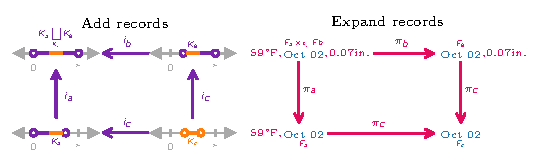
\includegraphics[width=\textwidth]{more_records.pdf}
\caption{Pullback (left) and pushout (right) structure of the operations that add records (increasing the indexing base space) or expand records (merging different fiber spaces with a database join-like operation).}\label{fig:more-records}
\end{figure*}


\begin{figure*}[h]
    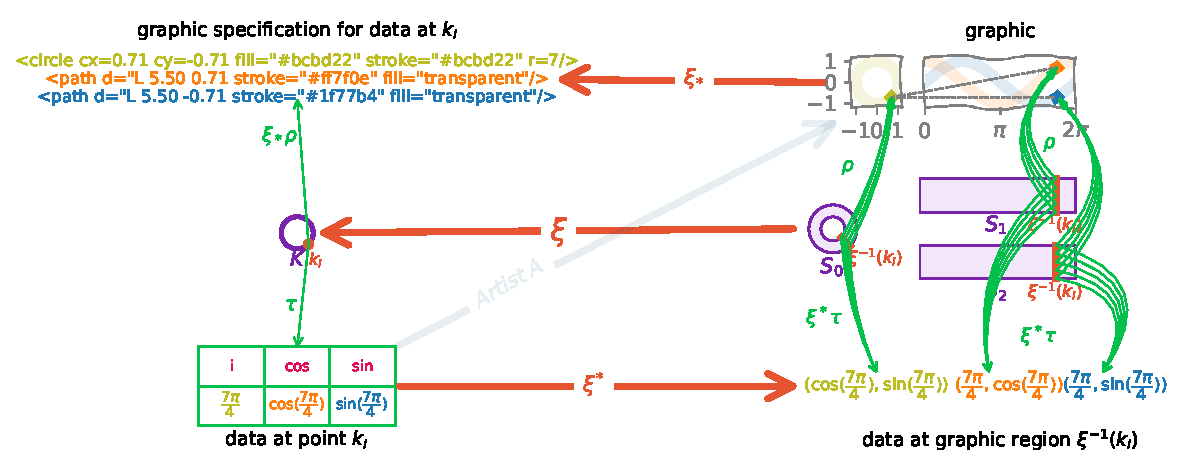
\includegraphics[width=7.16in]{xi_diagram.pdf}
    \caption{A deformation retract $\vindexc$ that relates the graphics footprint $S_0$ of an abstract circle to the circle itself gives rise to a pair of additional maps. The pushforward $\vindexpushc$ matches a point in the graphical realization to the specification of the graphic at that point, while the pullback $\vindexpullc$ matches each point in the graphic space to the data giving rise to that point.
    }
    \label{fig:xi}
\end{figure*}

As illustrated in \autoref{fig:xi}, this deformation retract $\vindexc$ gives rise to two so-called transport functors $(\vindexpush, \vindexpull)$ -- known as the pushforward $\vindexpushc$ and pullback\footnote{different use of the word pullback than in the preceding paragraph -- an unfortunate collision of terminology} $\vindexpullc$. These also codify how visual elements correspond to distinct data elements, which is a necessary condition of a visualization being readable\cite{ziemkiewiczEmbeddingInformationVisualization2009}. The pushforward $\vindexpushc$ matches each point in the data space to the specification of the graphic at that point $\vindexpushc\gsectionc(\dbasepointc) = \gsectionc\restriction_{\vindexprec(\dbasepointc)}$, while the pullback $\vindexpull$ matches each point in the graphic space to the data over that point $\vindexpullc\dsectionc(\gbasepointc) = \dsectionc(\vindexc(\gbasepointc)) = \dsectionc(\dbasepointc)$.




\section{Construction}

Artists naturally factorize into a two-stage process, starting with an encoding stage $\vchannelc$ followed by a compositing stage $\vmarkc$. In the \textcolor{artist}{encoding} stage $\vchannelc$, a data bundle is mapped to a visual variable bundle \vchannel, where the fibers of \vchannel\ are an internal library specification of graphics. The \textcolor{artist}{compositing} stage $\vmarkc$ then assembles the visual components into a visual element.


\section{Conclusion}

We have demonstrated a mathematical formalism for representing a data visualization pipeline, in which the mathematical structures both enforce well known principles of data visualization and suggest factorizations and decompositions resulting in a highly modularizable infrastructure, where artists can be constructed from composable primitive. This decomposability leads directly to a test framework ambition: if we can split $A=\vmarkc\circ\vchannelc$, and each factor $\vchannelc$, $\vmarkc$ can be further decomposed into composable primitives, we can focus testing on each of these building blocks reducing testing for correctness of the process as a whole to correctness of each building block, and correctness of their chosen combinations.

Furthermore, while the graphics sheaves here deal with visual properties -- pixel positions and colors, et.c. -- one could easily imagine picking a different choice for the fiber $\gfiberc$ in the realization sheaf that tracks information about haptic or auditory expressions, resulting in an identical abstraction, with many overlapping building blocks, for multimodal data representations.


\section*{Note}
This is a work in progress, more information can be found at https://github.com/story645/team

\section*{Acknowledgements}
The authors would like to thank the anonymous reviewers who gave constructive feedback on an earlier version of this paper. The authors are also grateful to  the various Matplotlib and Napari contributors, particularly Juan Nunez-Iglesias, and Nicolas Kruchten for their valuable feedback from the library developer perspective. Hannah is also very grateful to Nicolas for the suggestion of augmented notation and to the nlab and wikipedia contributors who wrote clear explanations of many of the topics discussed in this paper. This project has been made possible in part by grant number 2019-207333 (EOSS Cycle 1) and EOSS Cycle 3 Chan Zuckerberg Initiative DAF, an advised fund of Silicon Valley Community Foundation


\bibliographystyle{plain}
\bibliography{references}
\end{document}
